\chapter{Caso de uso: \#BLM}
\label{chap:casouso}

Para mostrar el funcionamiento de la aplicación, a lo largo de este capítulo se desarrollará un caso de uso real y se irá
comentando paso a paso.

\section{Puesta en marcha del sistema}

Como se mencionó en la Sección \ref{sec:herramientas_soporte}, para poder ejecutar la aplicación simplemente es necesario tener
instalado Docker y Docker-Compose. Una vez instalados, es necesario ejecutar el siguiente comando en la raíz del
proyecto:

\bigskip
\begin{Verbatim}
docker-compose up
\end{Verbatim}

\bigskip
A partir de este momento, Docker se encargará de descargar las imágenes necesarias para ejecutar la aplicación y de levantar los
contenedores. Una vez finalizado el proceso, se podrá acceder a la aplicación de forma local en la URL: \url{http://localhost:3000}.

\section{\textit{Dataset} del movimiento BLM}

Como se comentó en el Capítulo \ref{chap:introduccion}, en las redes sociales se genera una gran cantidad de información y se debate sobre
diversos temas. Por ello, numerosos investigadores han utilizado esta información para crear lo que se conoce como "archivos sociales"
(Pybus et al., 2015 \cite{pybus2015hacking}; Acker et al., 2014 \cite{acker2014death}; Ruiz et al., 2020 \cite{ruiz2020cuentalo}),
que buscan preservar determinados aspectos de la interacción en las redes sociales y servir como base para futuras investigaciones
y estudios.

\bigskip
En este contexto, los tutores de este trabajo, utilizando una metodología propia para la creación de colecciones de referencia
a modo de archivos sociales
(Otero et al., 2021 \cite{oterorodilla2021}), han elaborado un \textit{dataset} sobre el fenómeno social
que se produjo tras la muerte de George Floyd en mayo de 2020 conocido como \textit{Black Lives Matter},
que implicó protestas en todo el mundo en las que se denunciaba la brutalidad policial y el racismo sistémico en Estados Unidos. Esta colección, 
disponible tanto en español como en inglés, recoge más de 260.000 posts referentes a más de 90.000 usuarios de la red social Reddit que compartieron contenido sobre este
fenómeno en el periodo de aproximadamente un año.

\bigskip
Sin emabargo, debido a que la colección estaba formada por varios archivos diferentes en formato XML, donde unos contenían información de los hilos
de conversación en Reddit y otros posts de los usuarios que interactuaban en dichos hilos, fue necesario procesarlos y unificarlos
en un \textit{dataset} con un formato sencillo y aceptado por la aplicación. Así, se generaron tres \textit{datasets}, todos ellos
en inglés, en formato NDJSON, cada uno con 
un número diferente de posts para cada usuario (50, 500 y 1000) con el fin de analizar las posibles diferencias en cuanto a los resultados
obtenidos tras el perfilado.

\section{Subida del \textit{dataset}}

Una vez contamos con el \textit{dataset} que vamos a procesar para el perfilado, el primer paso es subirlo a la aplicación. Para ello,
en la página de inicio, mostrada en la Figura \ref{fig:casouso_home}, se puede observar, a mayores de un
campo de búsqueda por usuario de Twitter, un campo para la subida del \textit{dataset}, que será el que empleemos.
Destacar que, en este caso y a lo largo del resto de secciones de este capítulo,
se mostrarán las capturas de pantalla tanto de la versión de escritorio (izquierda) como de la versión móvil (derecha).

\bigskip
\begin{figure}[H]
	\centering
	\begin{subfigure}[c]{0.74\textwidth}
			\centering
			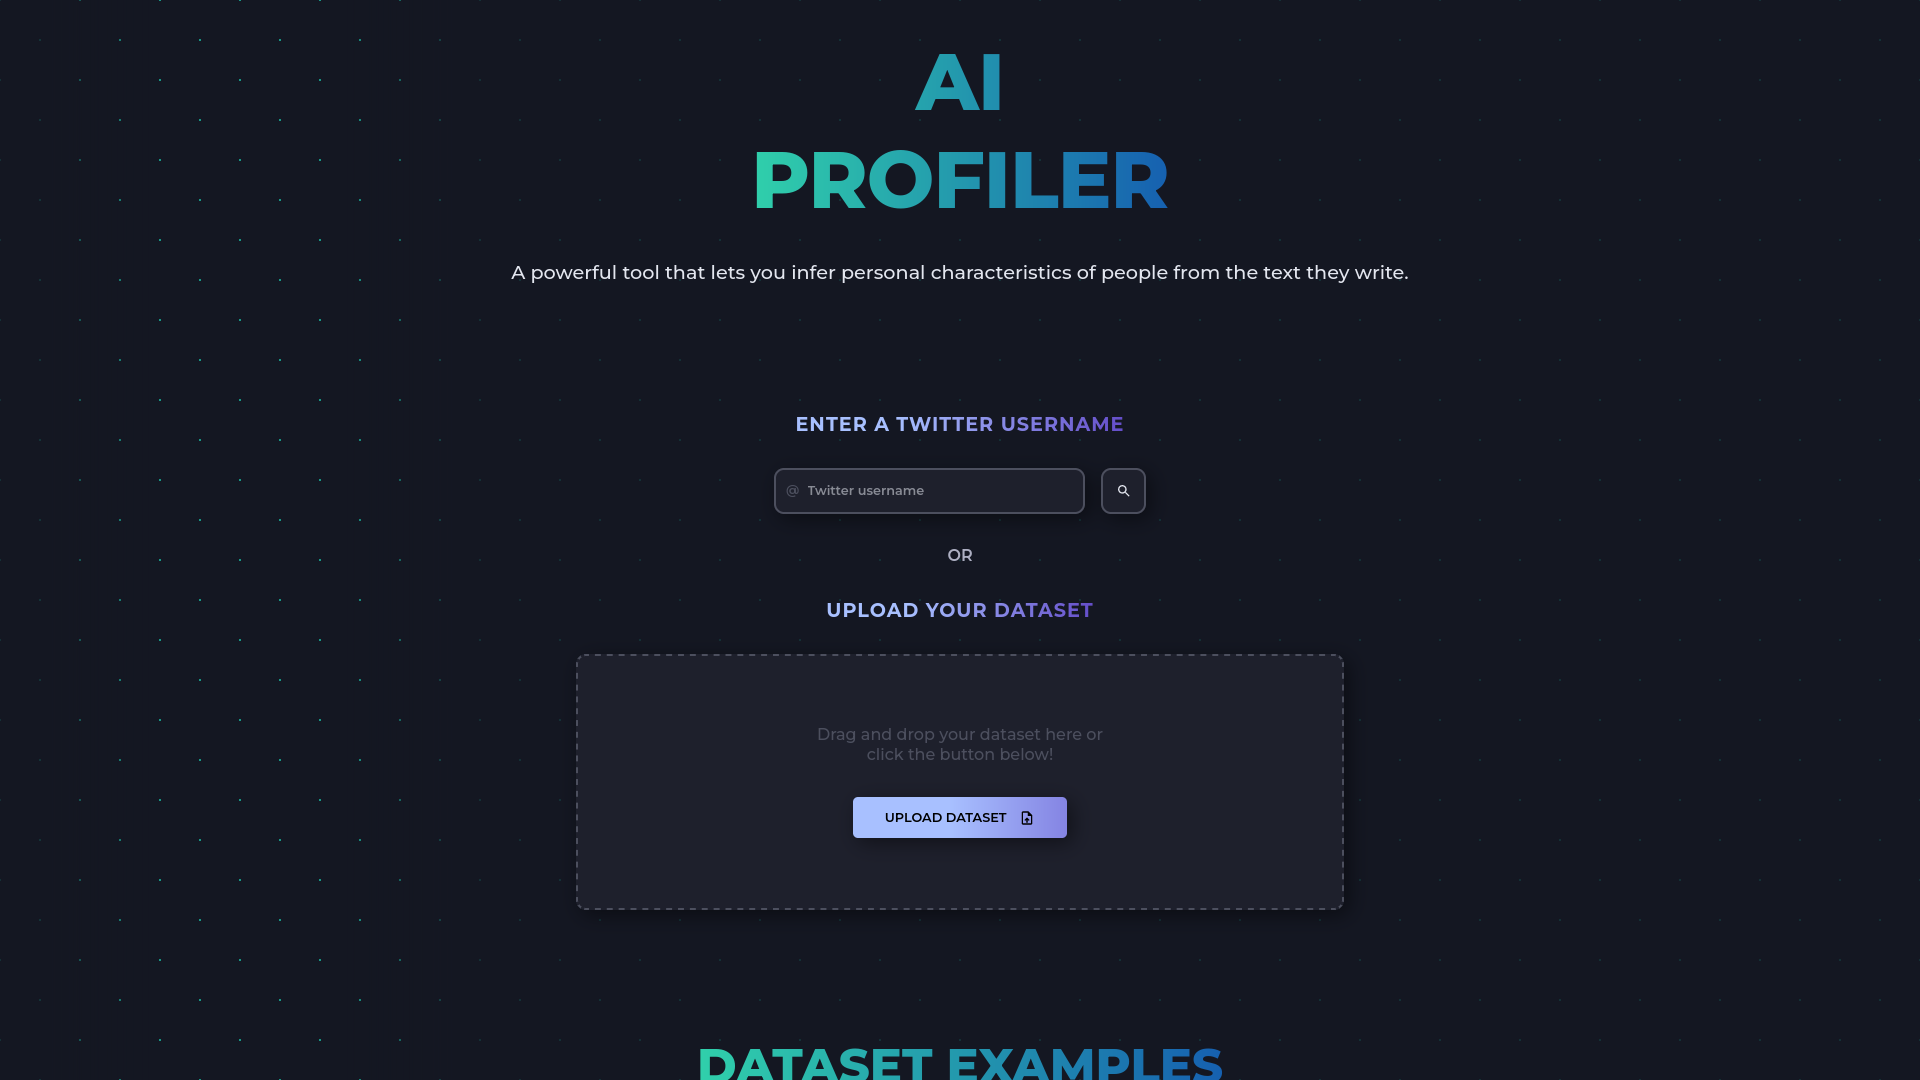
\includegraphics[width=\textwidth]{imagenes/home.png}
			\label{fig:casouso_home_escritorio}
	\end{subfigure}
	\hfill
	\begin{subfigure}[c]{0.21\textwidth}
			\centering
			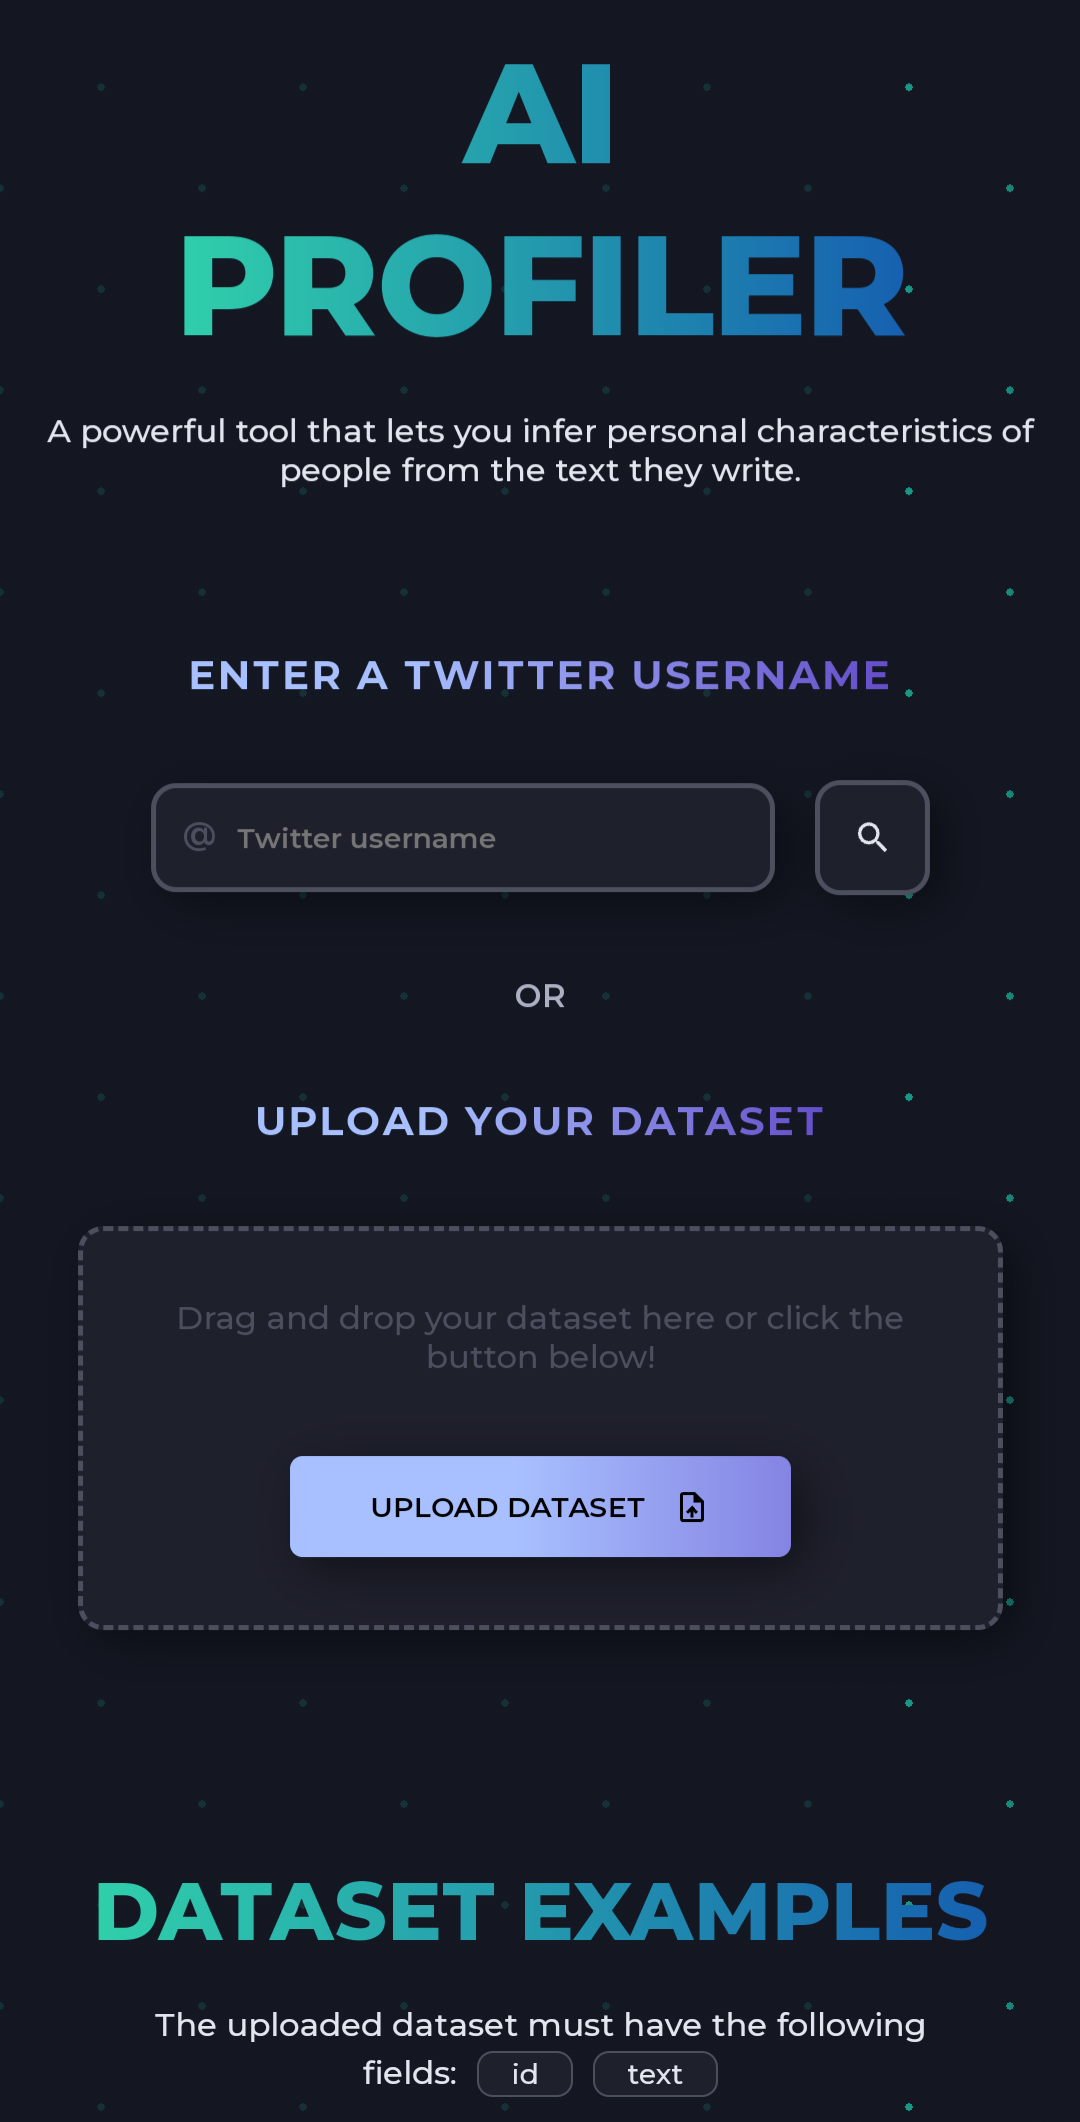
\includegraphics[width=\textwidth]{imagenes/home_movil.png}
			\label{fig:casouso_home_movil}
	\end{subfigure}
	\vspace{-1\baselineskip}
	\caption{Página de inicio de la aplicación}
	\label{fig:casouso_home}
\end{figure}

\bigskip
Asimismo, si el usuario desea conocer cual es la estructura y los campos que debe contener el \textit{dataset} que va a subir,
puede hacerlo consultando la sección de ejemplos, mostrada en la Figura \ref{fig:casouso_examples}, visible tras hacer \textit{scroll}
en la misma página de inicio.

\bigskip
\begin{figure}[H]
	\centering
	\begin{subfigure}[c]{0.74\textwidth}
			\centering
			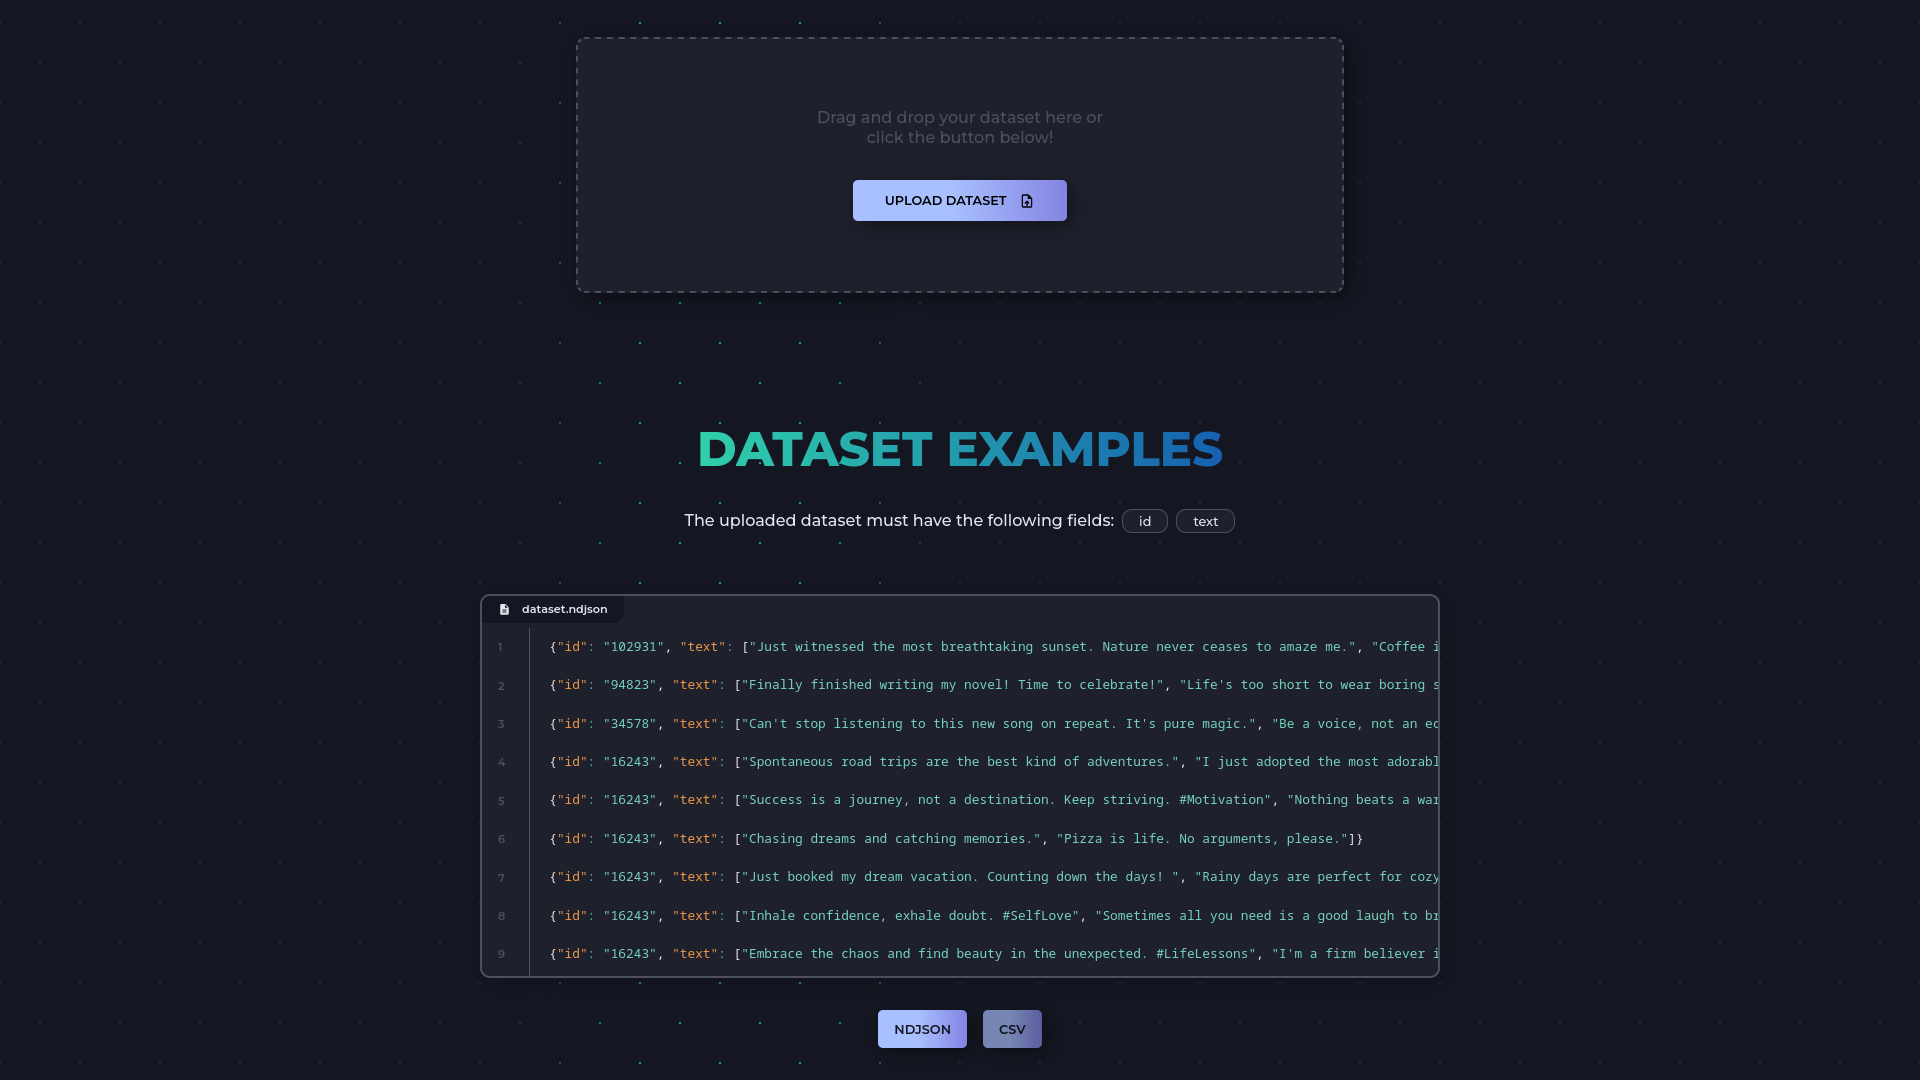
\includegraphics[width=\textwidth]{imagenes/examples.png}
			\label{fig:casouso_examples_escritorio}
	\end{subfigure}
	\hfill
	\begin{subfigure}[c]{0.21\textwidth}
			\centering
			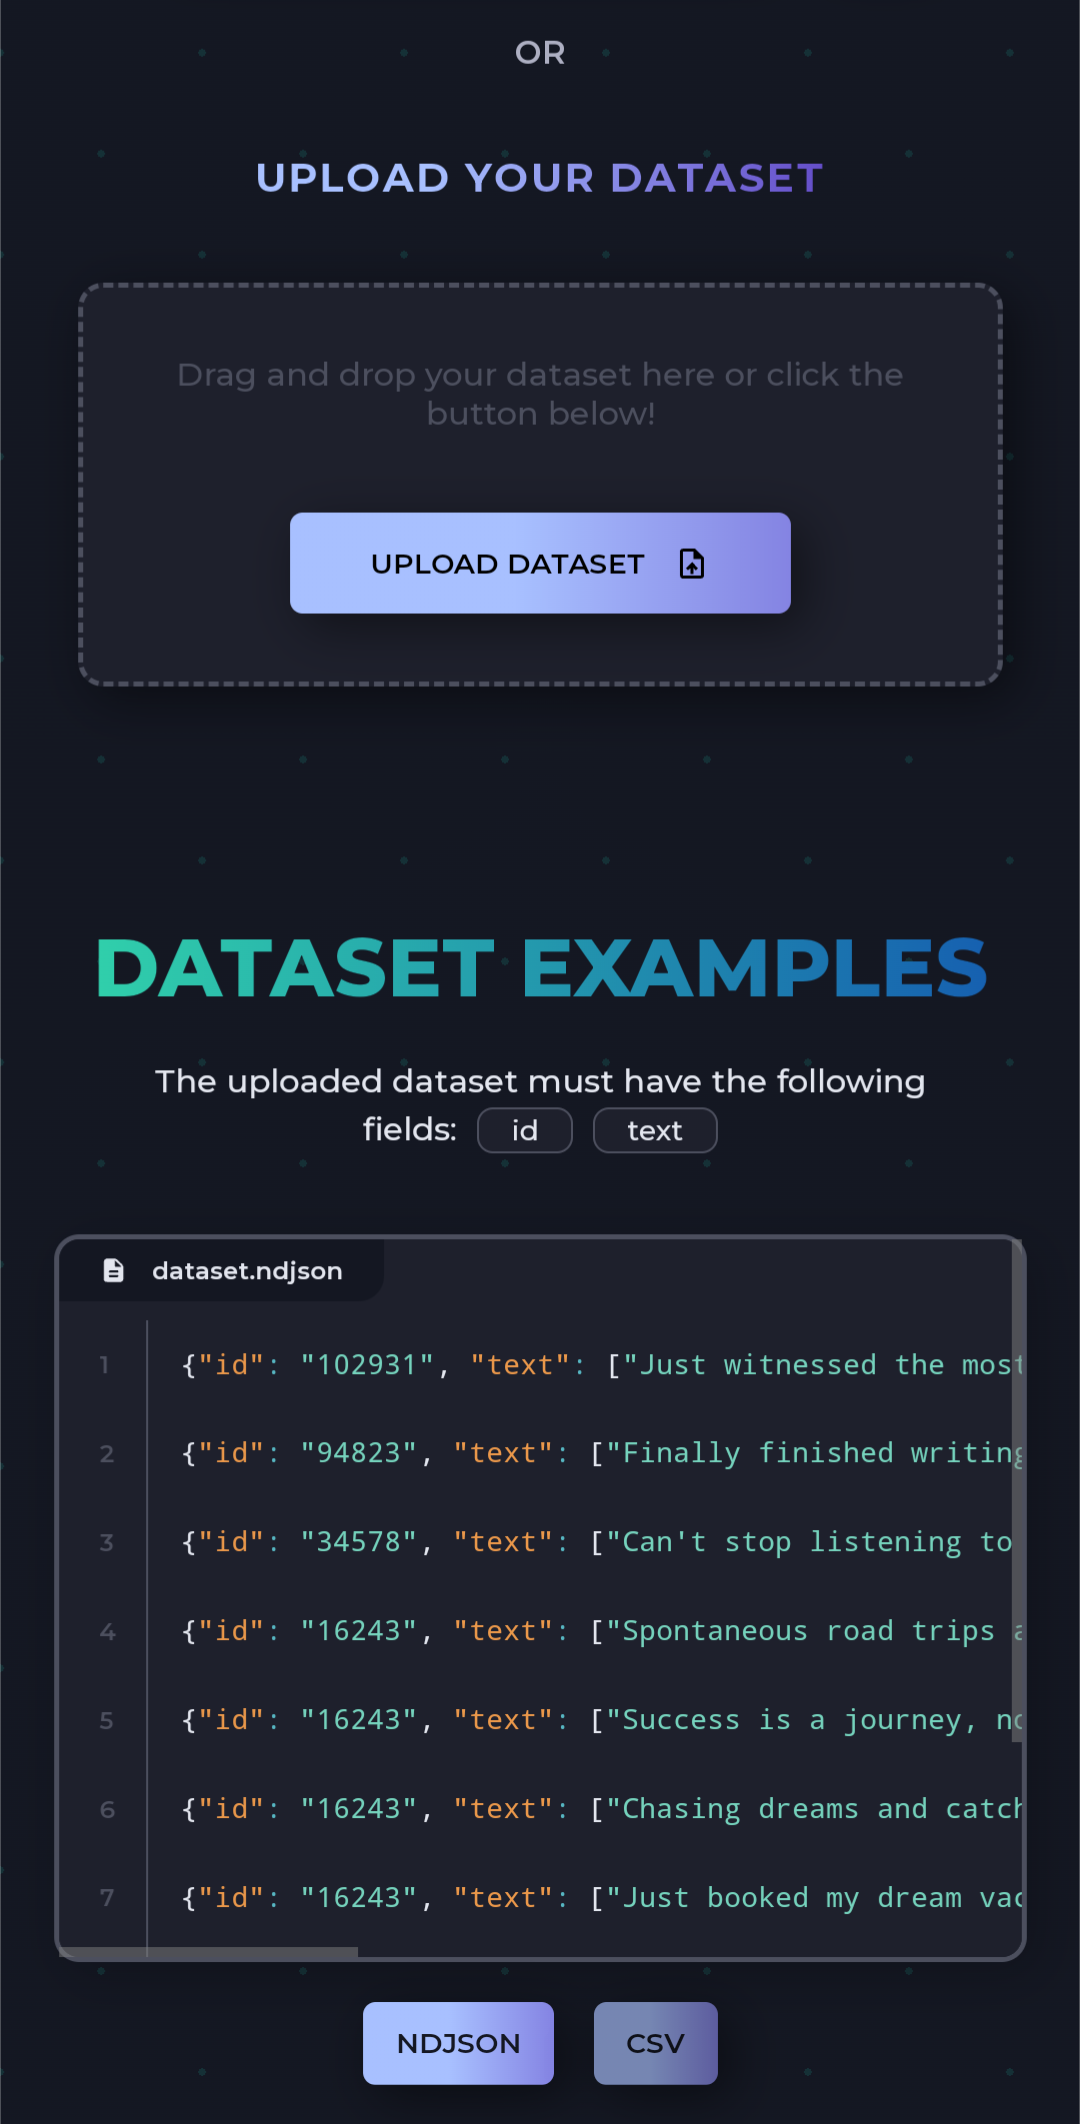
\includegraphics[width=\textwidth]{imagenes/examples_movil.png}
			\label{fig:casouso_examples_movil}
	\end{subfigure}
	\vspace{-1\baselineskip}
	\caption{Página de ejemplos de \textit{datasets}}
	\label{fig:casouso_examples}
\end{figure}

\section{Selección del algoritmo}

En este punto, una vez subido el \textit{dataset} deseado, el usuario debe seleccionar el algoritmo de perfilado que más se ajuste
a sus necesidades. En este decisión, es fundamental tener en cuenta el lenguaje en el que se encuentra el \textit{dataset},
las caracterísitcas que se buscan perfilar, el rendimiento del algoritmo o incluso el \textit{dataset} con el que ha sido entrenado.
Así, por un lado se muestran unas tarjetas con la información básica de cada algoritmo, como se puede ver
en la Figura \ref{fig:casouso_algorithms} y, por otro lado, se muestran \textit{tooltips} con información más detallada
sobre el funcionamiento del algoritmo, el \textit{dataset} de entrenamiento y el rendimiento del mismo, 
como se distingue en la Figura \ref{fig:casouso_tooltip}.

\bigskip
\begin{figure}[H]
	\centering
	\begin{subfigure}[c]{0.74\textwidth}
			\centering
			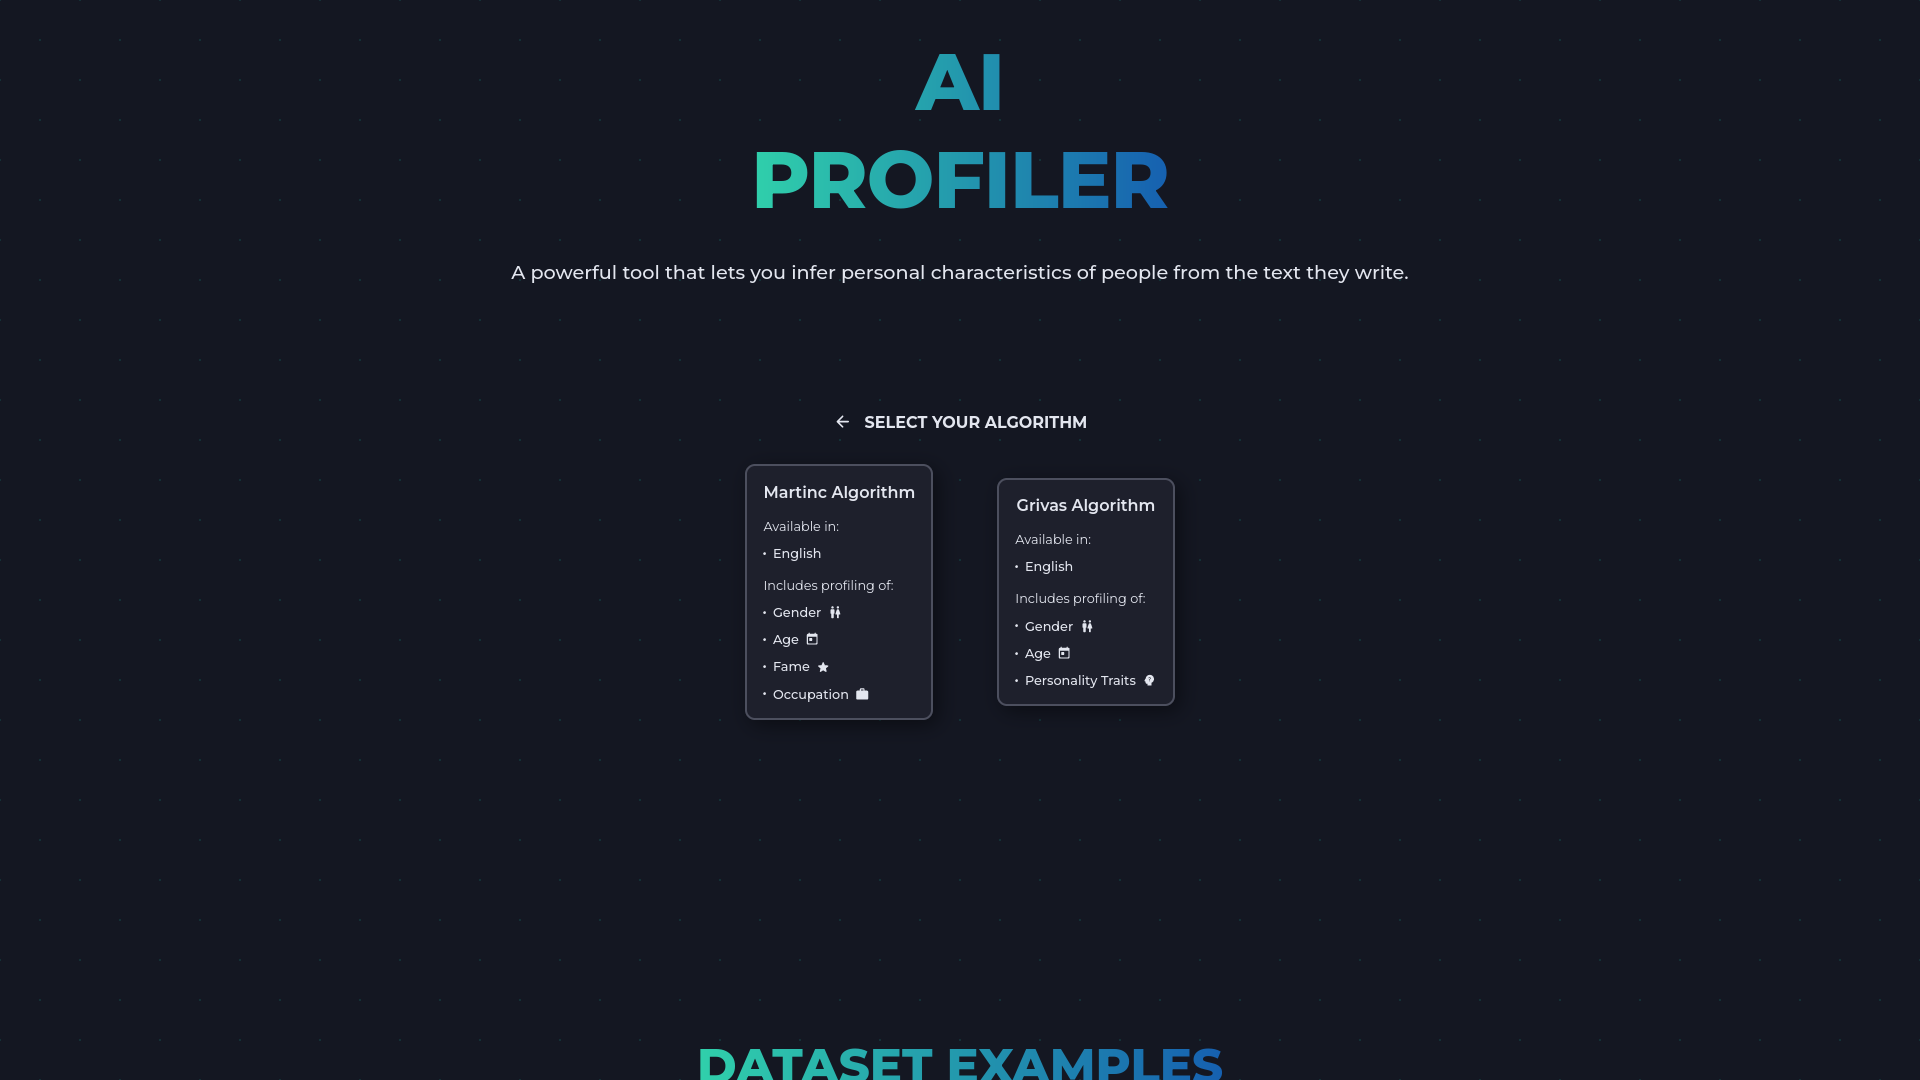
\includegraphics[width=\textwidth]{imagenes/algorithms.png}
			\label{fig:casouso_algorithms_escritorio}
	\end{subfigure}
	\hfill
	\begin{subfigure}[c]{0.21\textwidth}
			\centering
			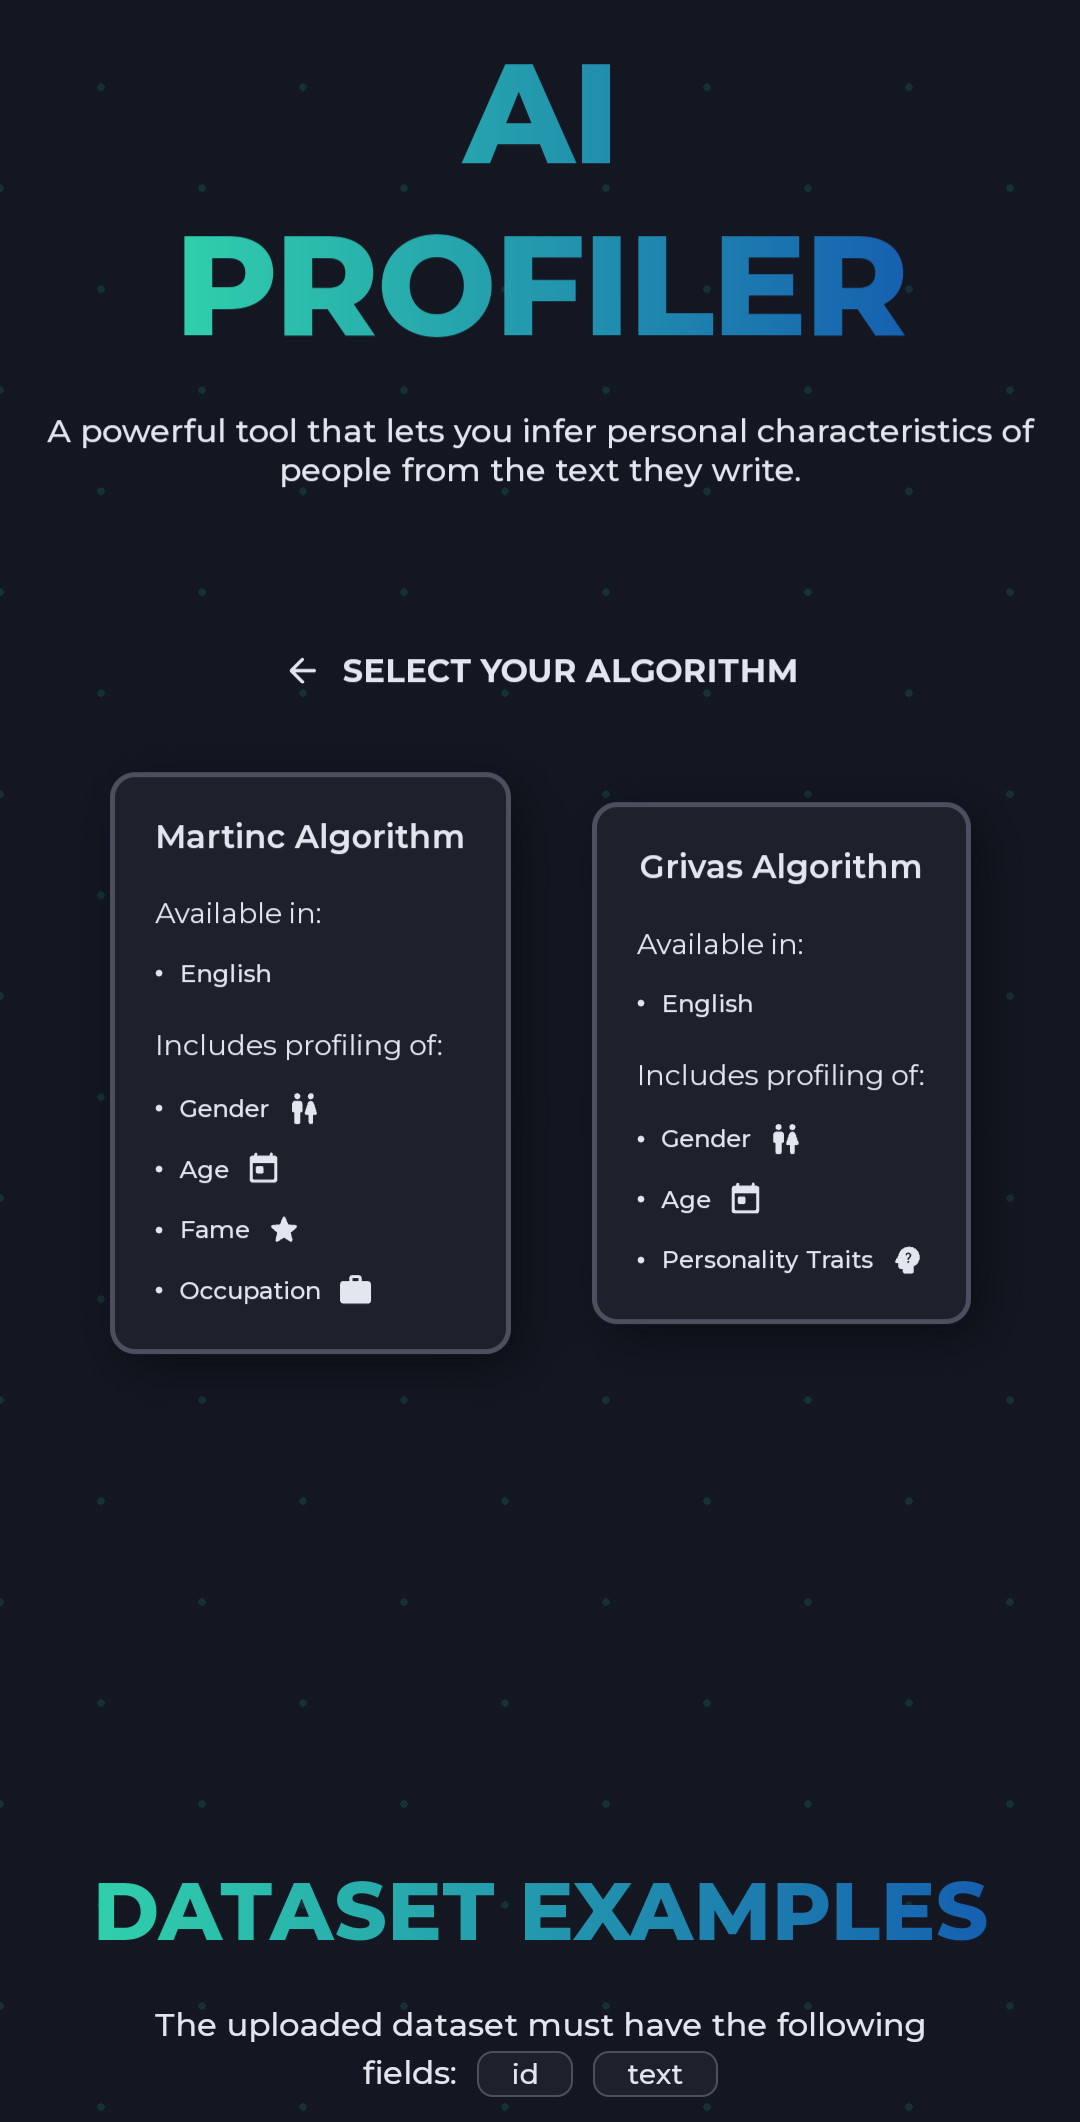
\includegraphics[width=\textwidth]{imagenes/algorithms_movil.png}
			\label{fig:casouso_algorithms_movil}
	\end{subfigure}
	\vspace{-1\baselineskip}
	\caption{Página de selección algoritmos}
	\label{fig:casouso_algorithms}
\end{figure}

\begin{figure}[H]
	\centering
	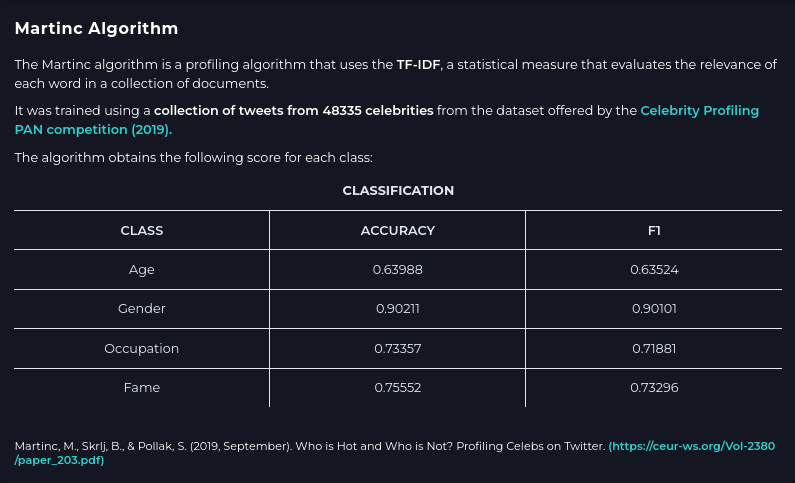
\includegraphics[width=0.5\textwidth]{imagenes/tooltip_only.png}
	\caption{Tooltip de información sobre el algoritmo}
	\label{fig:casouso_tooltip}
\end{figure}

\section{Proceso de perfilado}

Después de seleccionar el algoritmo, se muestra una página a modo de resumen, en la que se puede observar el \textit{dataset} subido
junto al algoritmo seleccionado. Para comenzar el proceso de perfilado, el usuario debe pulsar el botón
\textit{Start profiling} y, para proporcionar \textit{feedback} sobre la ejecución del proceso y mejorar la experiencia de usuario,
se muestra una barra de progreso infinita. Esta página puede verse en la Figura \ref{fig:casouso_overview}.

\bigskip
\begin{figure}[H]
	\centering
	\begin{subfigure}[c]{0.74\textwidth}
			\centering
			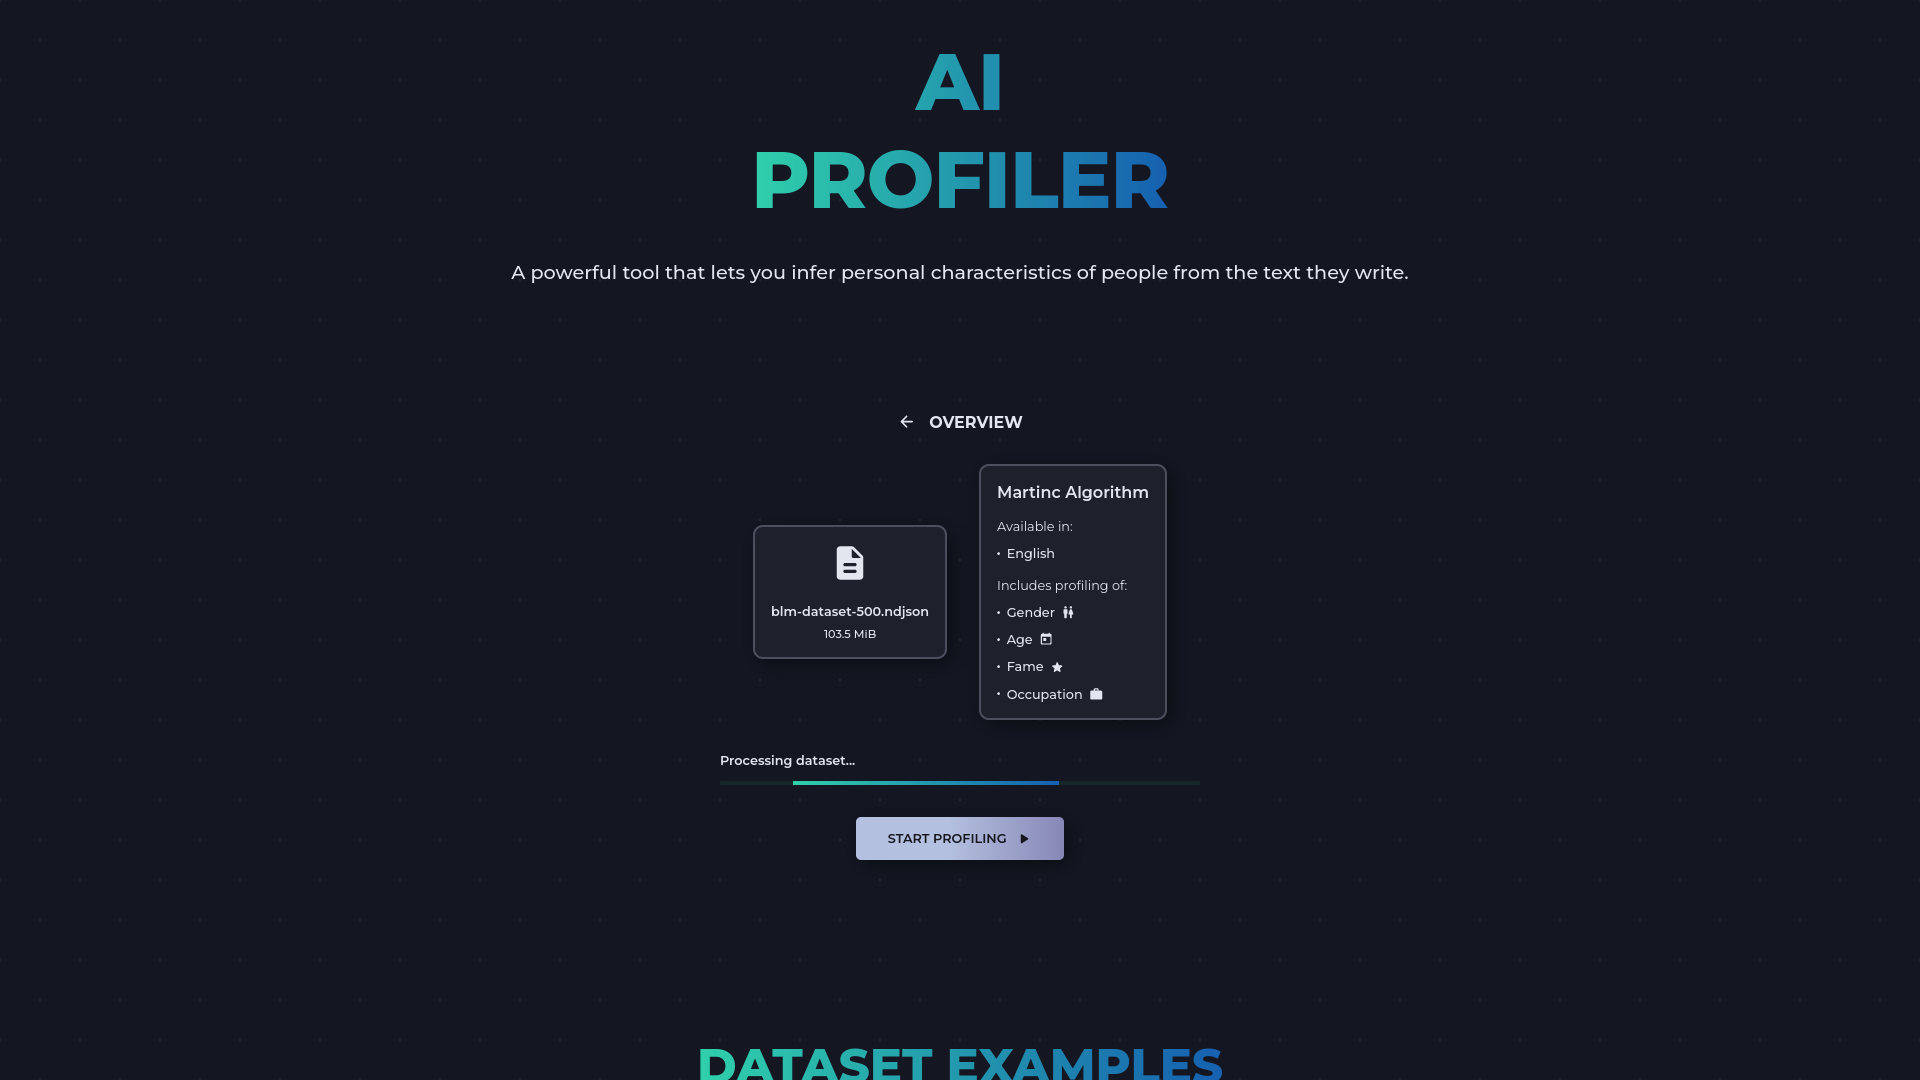
\includegraphics[width=\textwidth]{imagenes/overview.png}
			\label{fig:casouso_overview_escritorio}
	\end{subfigure}
	\hfill
	\begin{subfigure}[c]{0.21\textwidth}
			\centering
			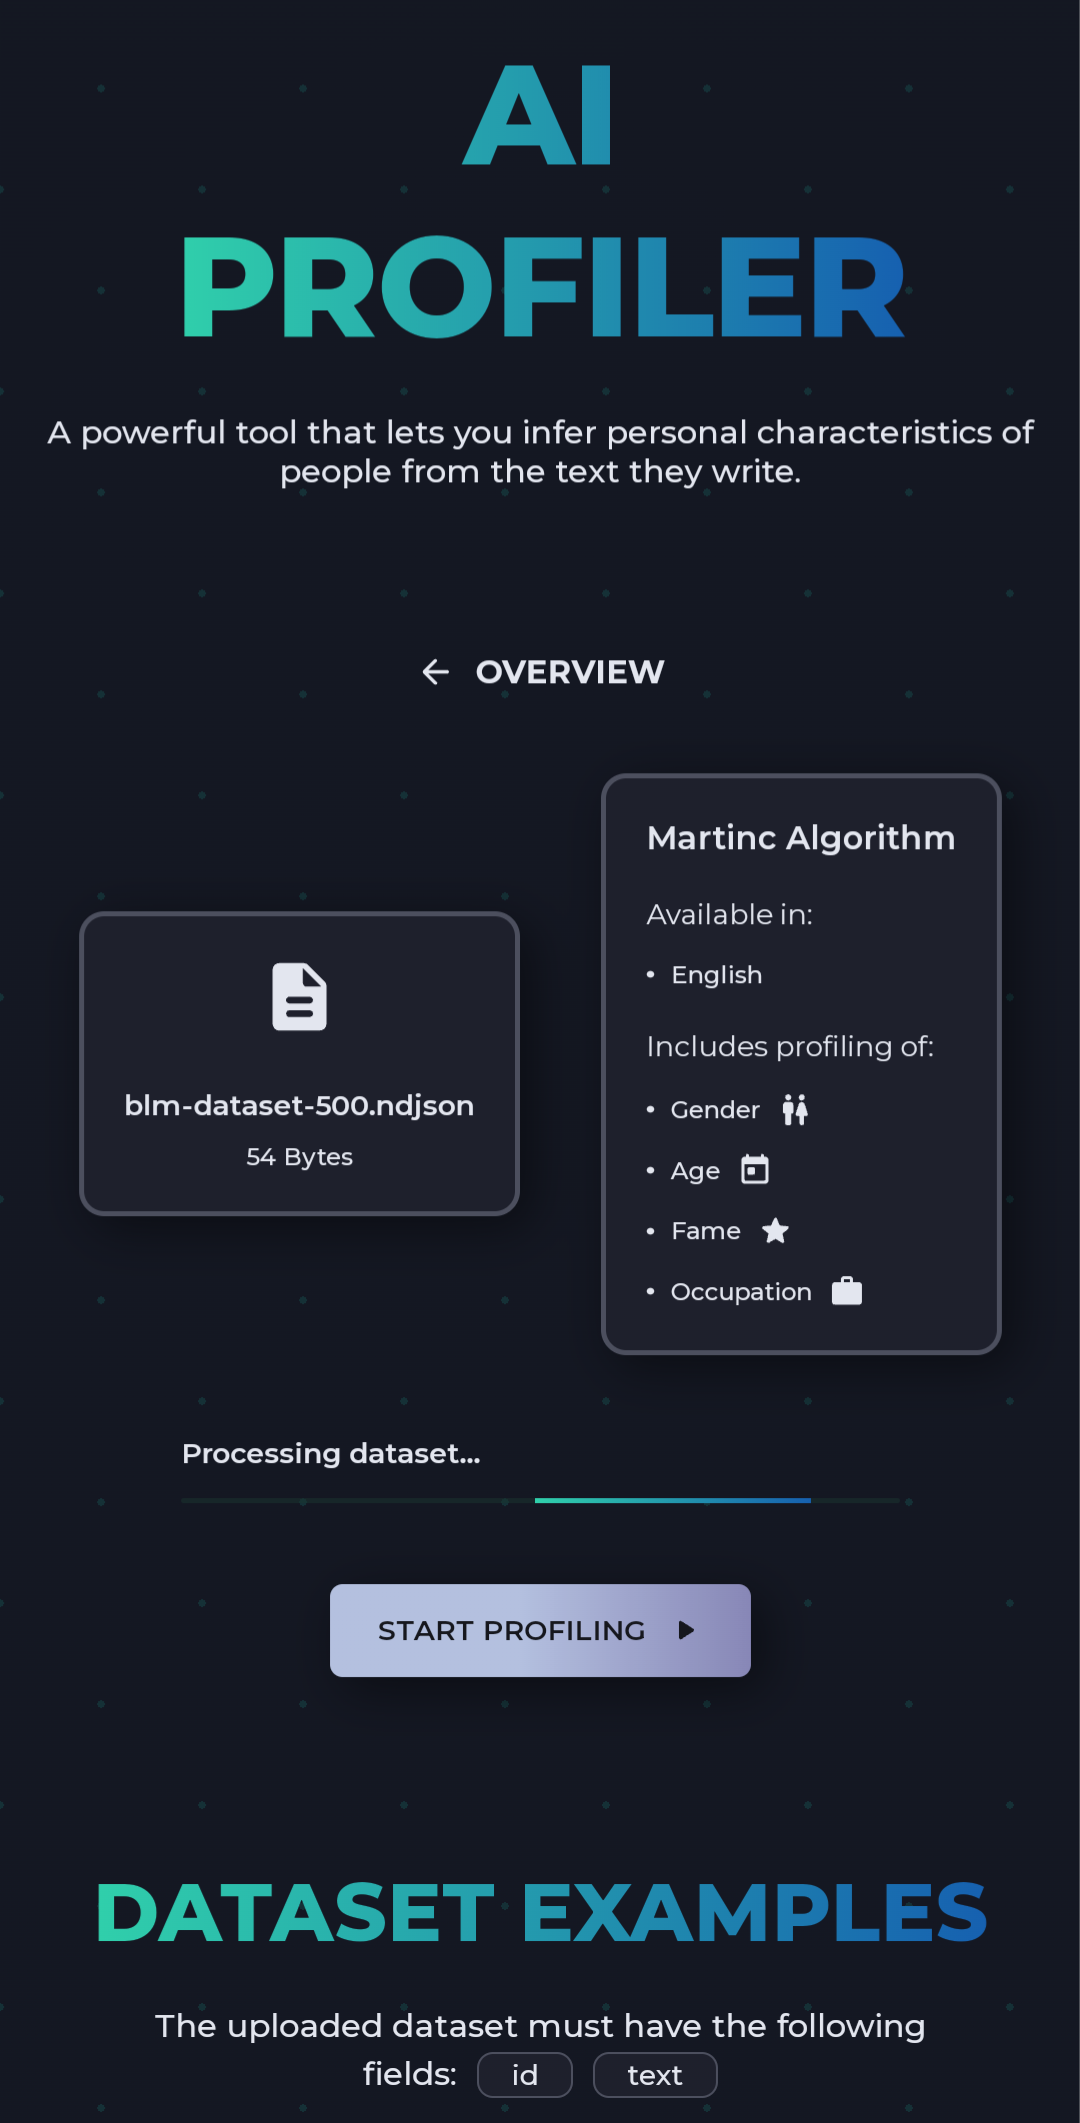
\includegraphics[width=\textwidth]{imagenes/overview_movil.png}
			\label{fig:casouso_overview_movil}
	\end{subfigure}
	\vspace{-1\baselineskip}
	\caption{Página de resumen del perfilado}
	\label{fig:casouso_overview}
\end{figure}

\section{Visualización de resultados}

Tras finalizar el proceso de perfilado, se muestra una página con los resultados obtenidos en formato \textit{dashboard}, al igual
que se especificaba en los prototipos de la Sección \ref{sec:diseño_prototipado}. De esta forma, el \textit{dashboard} fue
implementado teniendo como objetivo principal que toda la información estuviera disponible en una única página en la que se
mostraran únicamente datos relevantes para el usuario, sin necesidad de hacer \textit{scroll} para verla. Así, en función del algoritmo
empleado, se muestran unos gráficos u otros, como se puede ver en las Figuras \ref{fig:casouso_dashboard_martinc} y
\ref{fig:casouso_dashboard_grivas}.

\bigskip
\begin{figure}[H]
	\centering
	\begin{subfigure}[c]{0.74\textwidth}
			\centering
			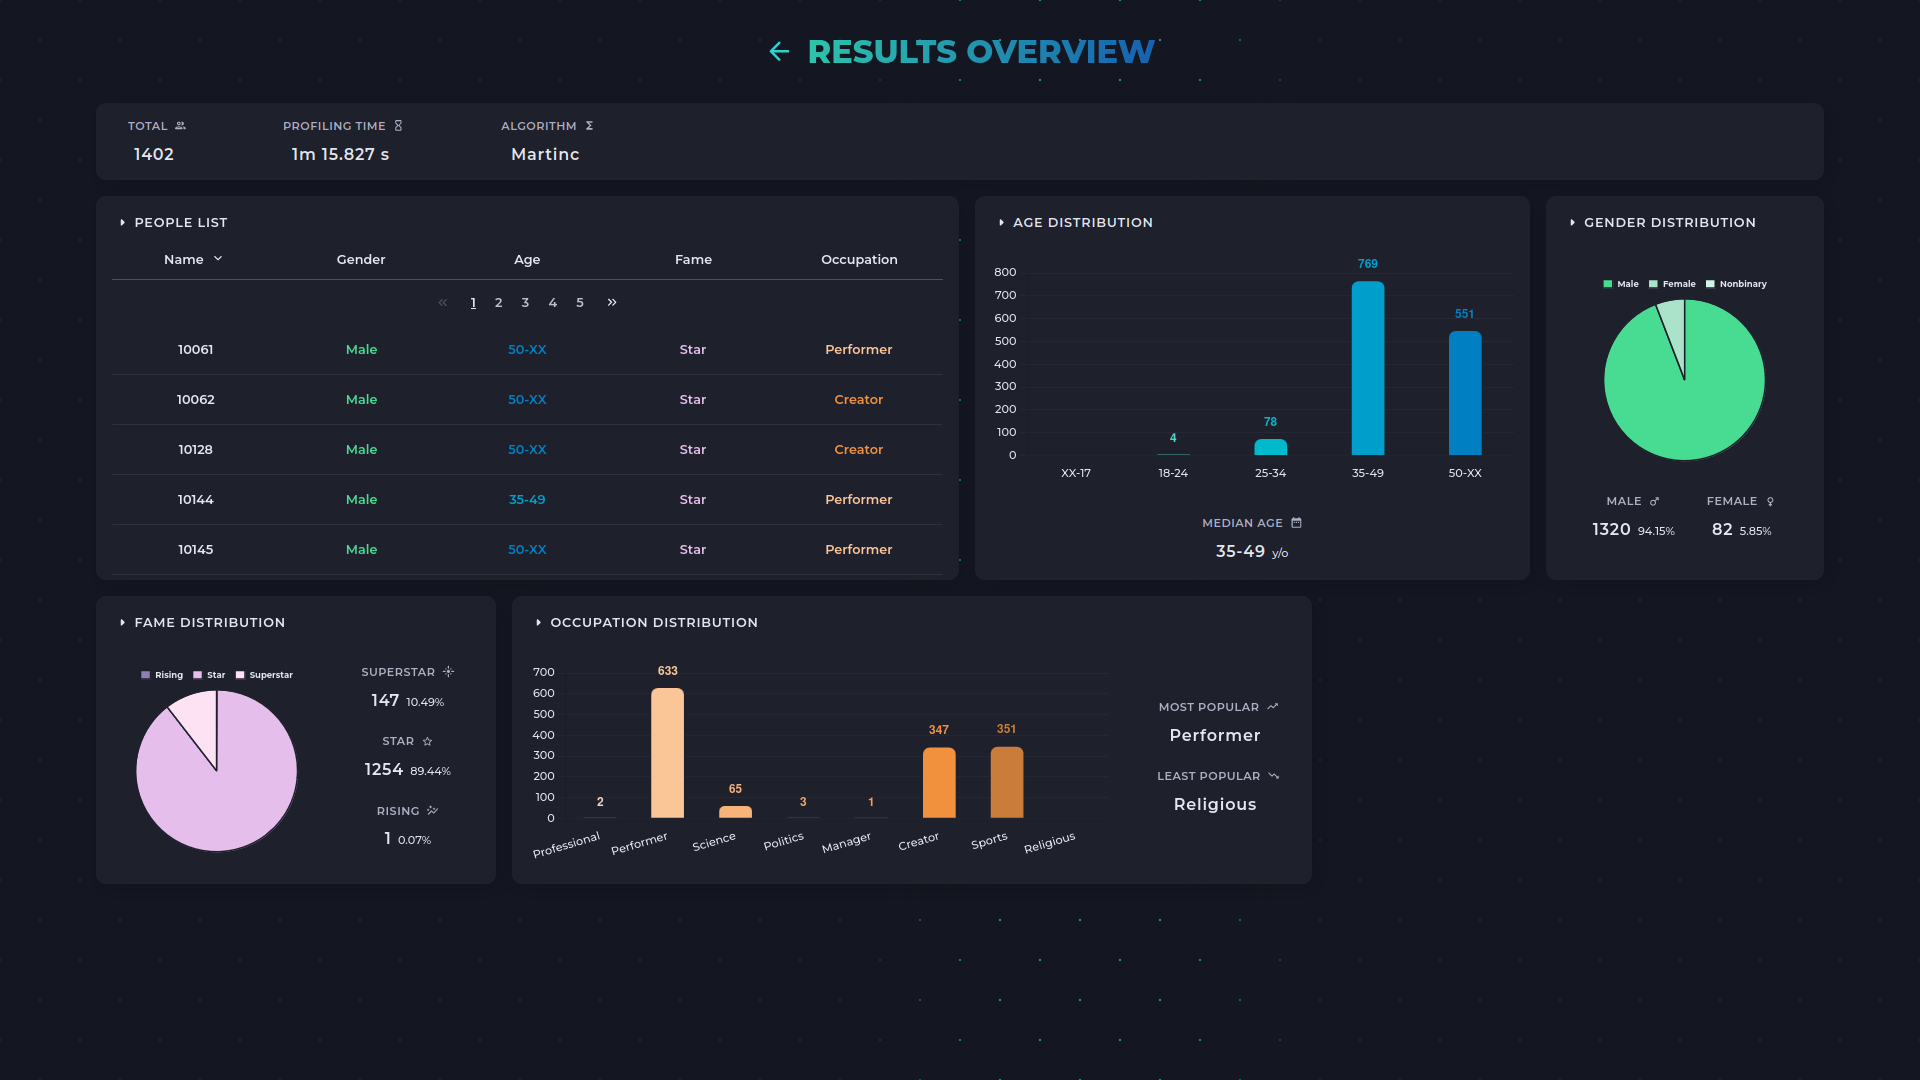
\includegraphics[width=\textwidth]{imagenes/dashboard-martinc-500.png}
			\label{fig:casouso_dashboard_martinc_escritorio}
	\end{subfigure}
	\hfill
	% \begin{subfigure}[c]{0.21\textwidth}
	% 		\centering
	% 		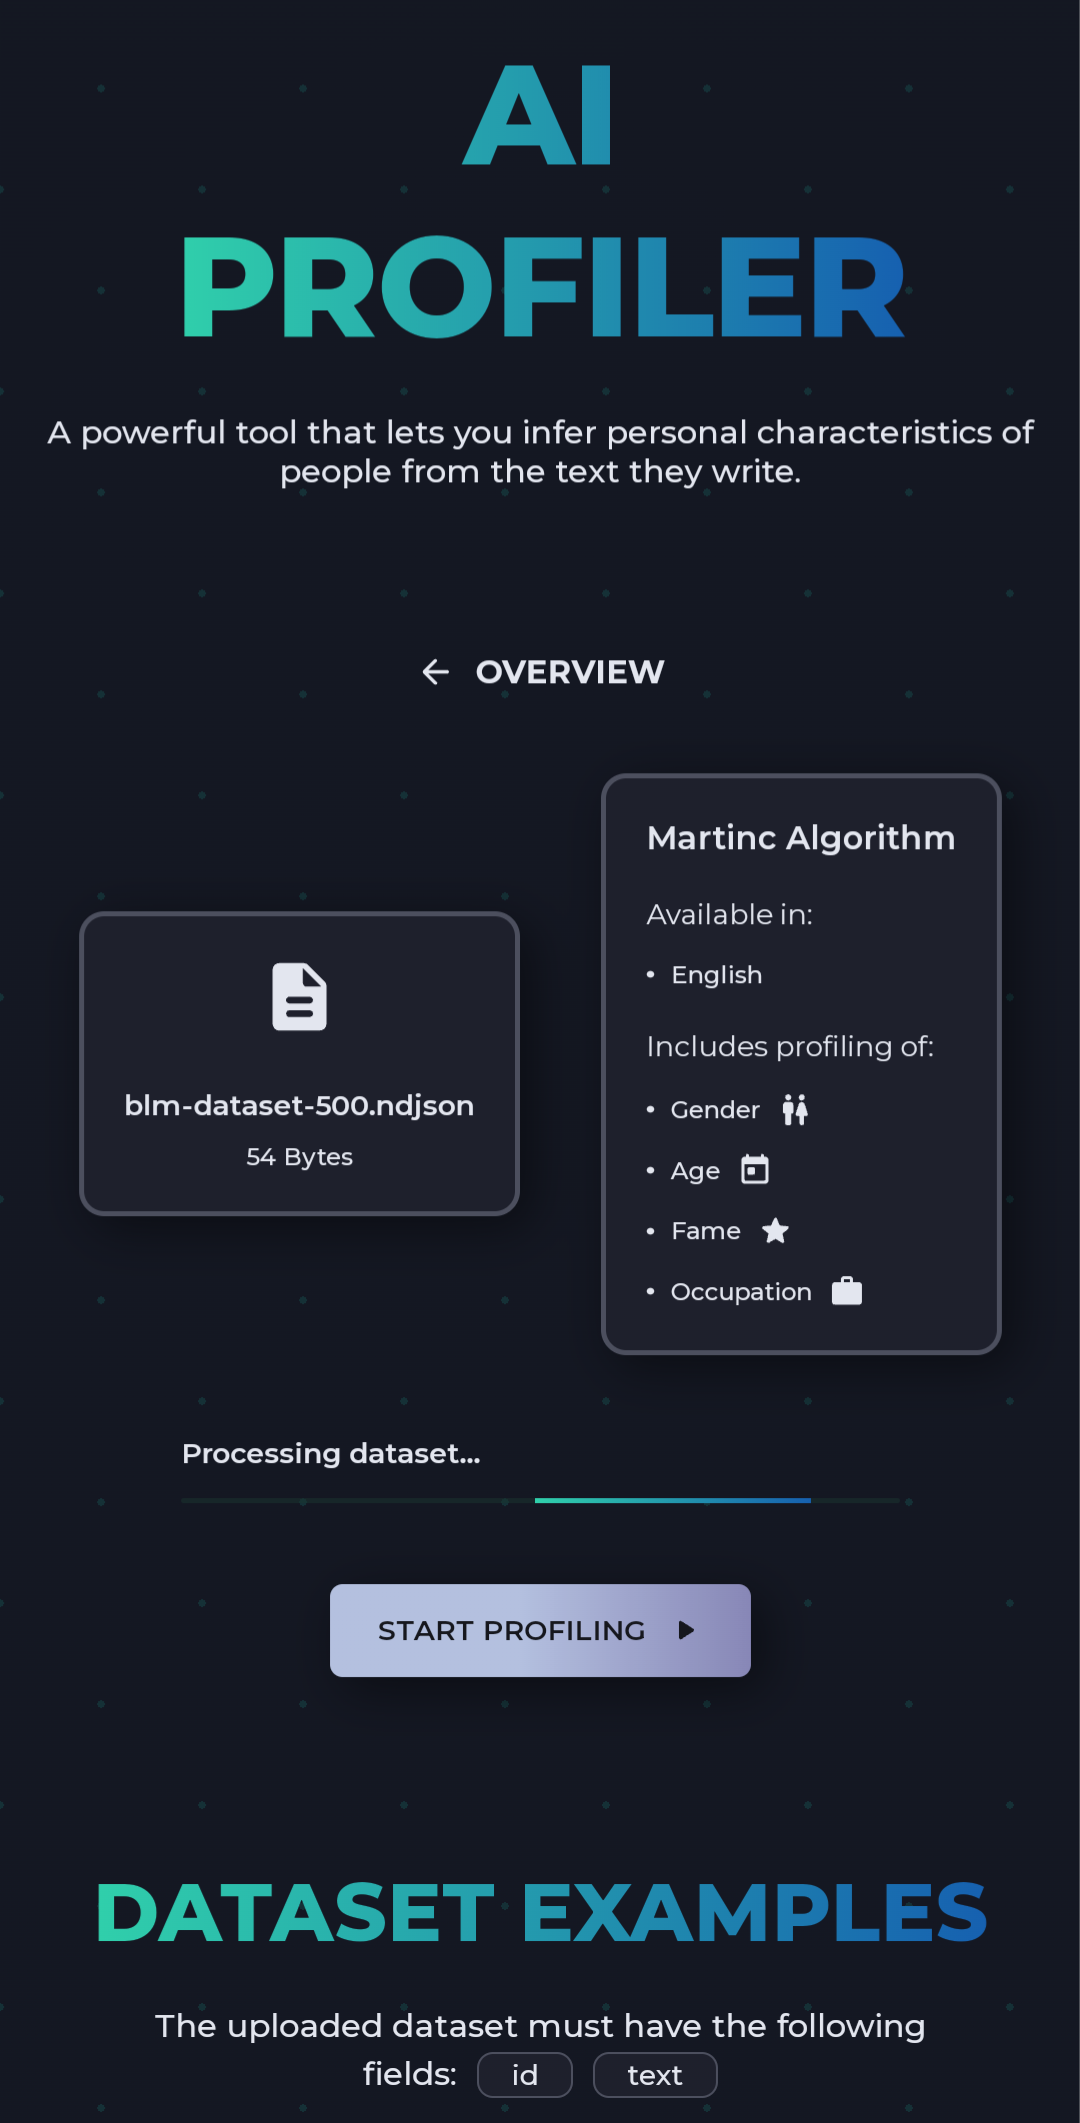
\includegraphics[width=\textwidth]{imagenes/overview_movil.png}
	% 		\label{fig:casouso_overview_movil}
	% \end{subfigure}
	\vspace{-1\baselineskip}
	\caption{Dashboard con los resultados obtenidos por el algoritmo de Martinc}
	\label{fig:casouso_dashboard_martinc}
\end{figure}

\begin{figure}[H]
	\centering
	\begin{subfigure}[c]{0.74\textwidth}
			\centering
			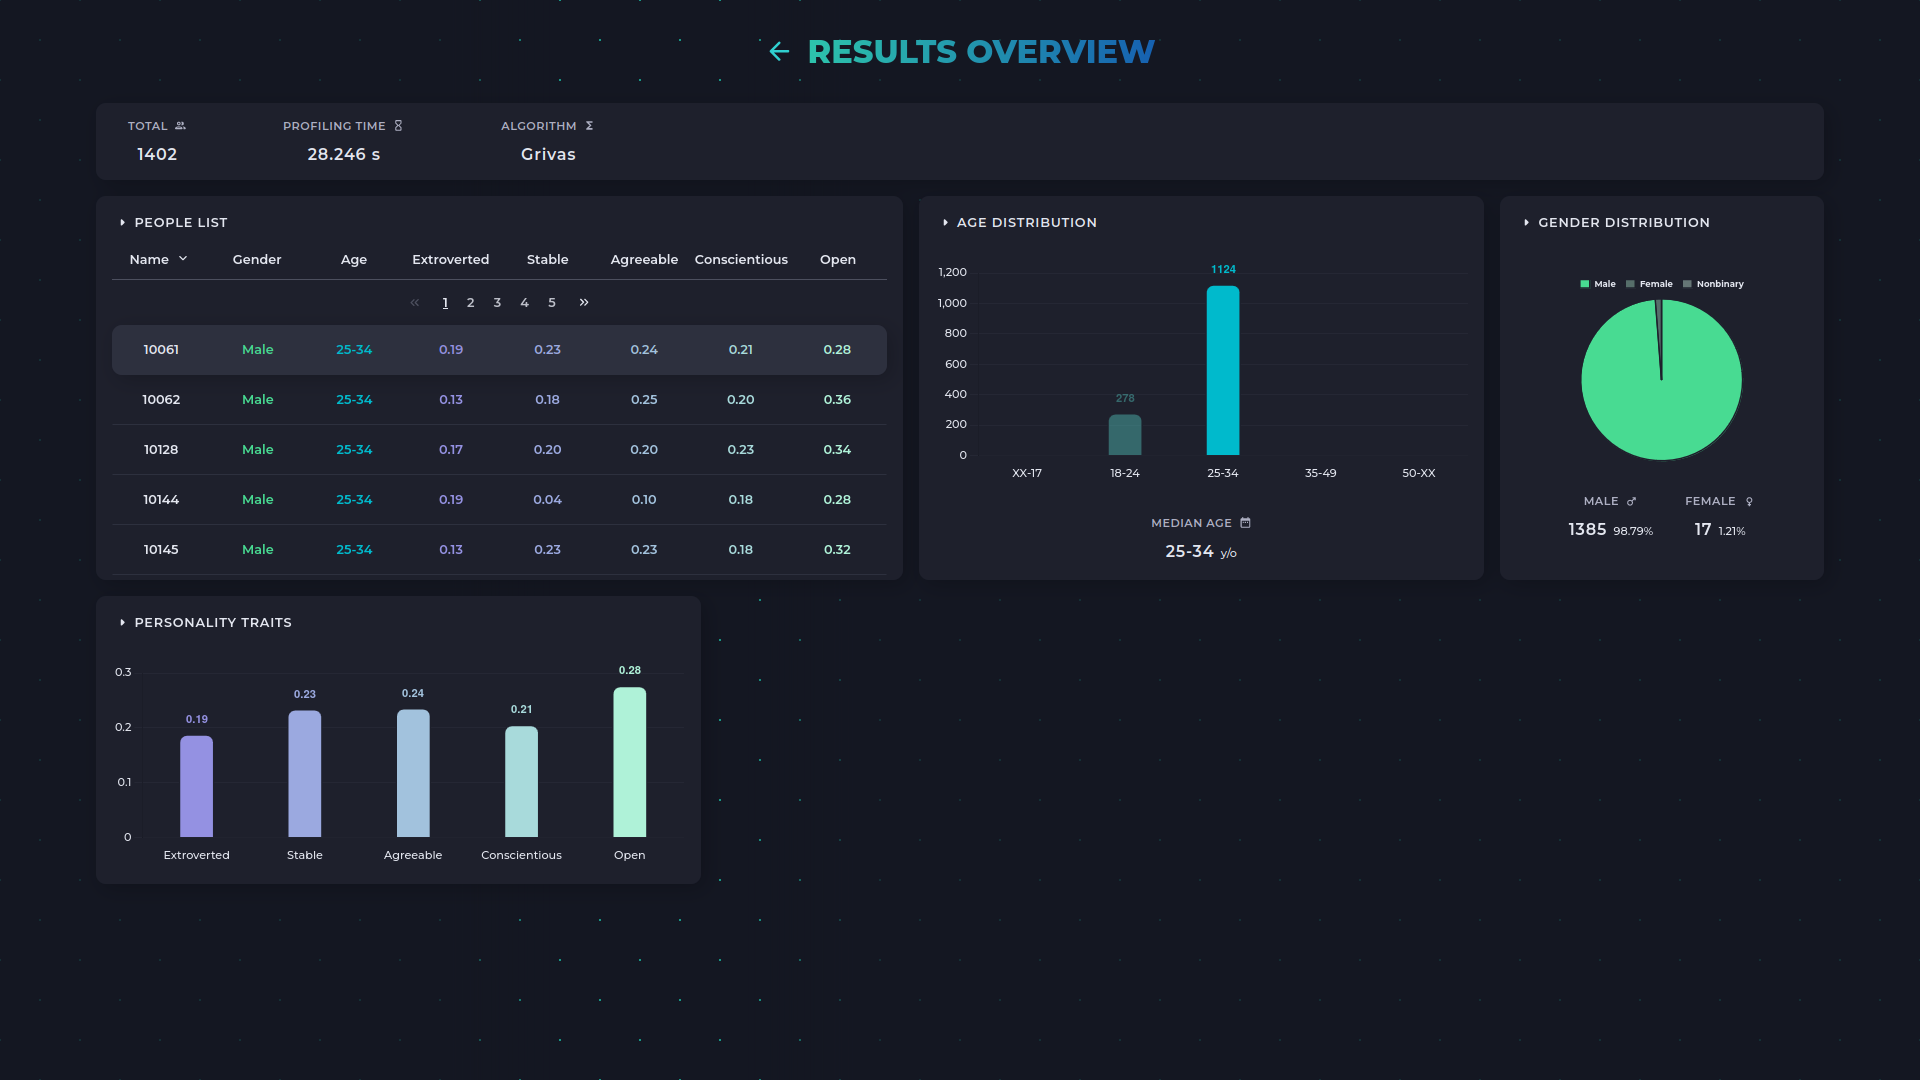
\includegraphics[width=\textwidth]{imagenes/dashboard-grivas-500.png}
			\label{fig:casouso_dashboard_grivas_escritorio}
	\end{subfigure}
	\hfill
	% \begin{subfigure}[c]{0.21\textwidth}
	% 		\centering
	% 		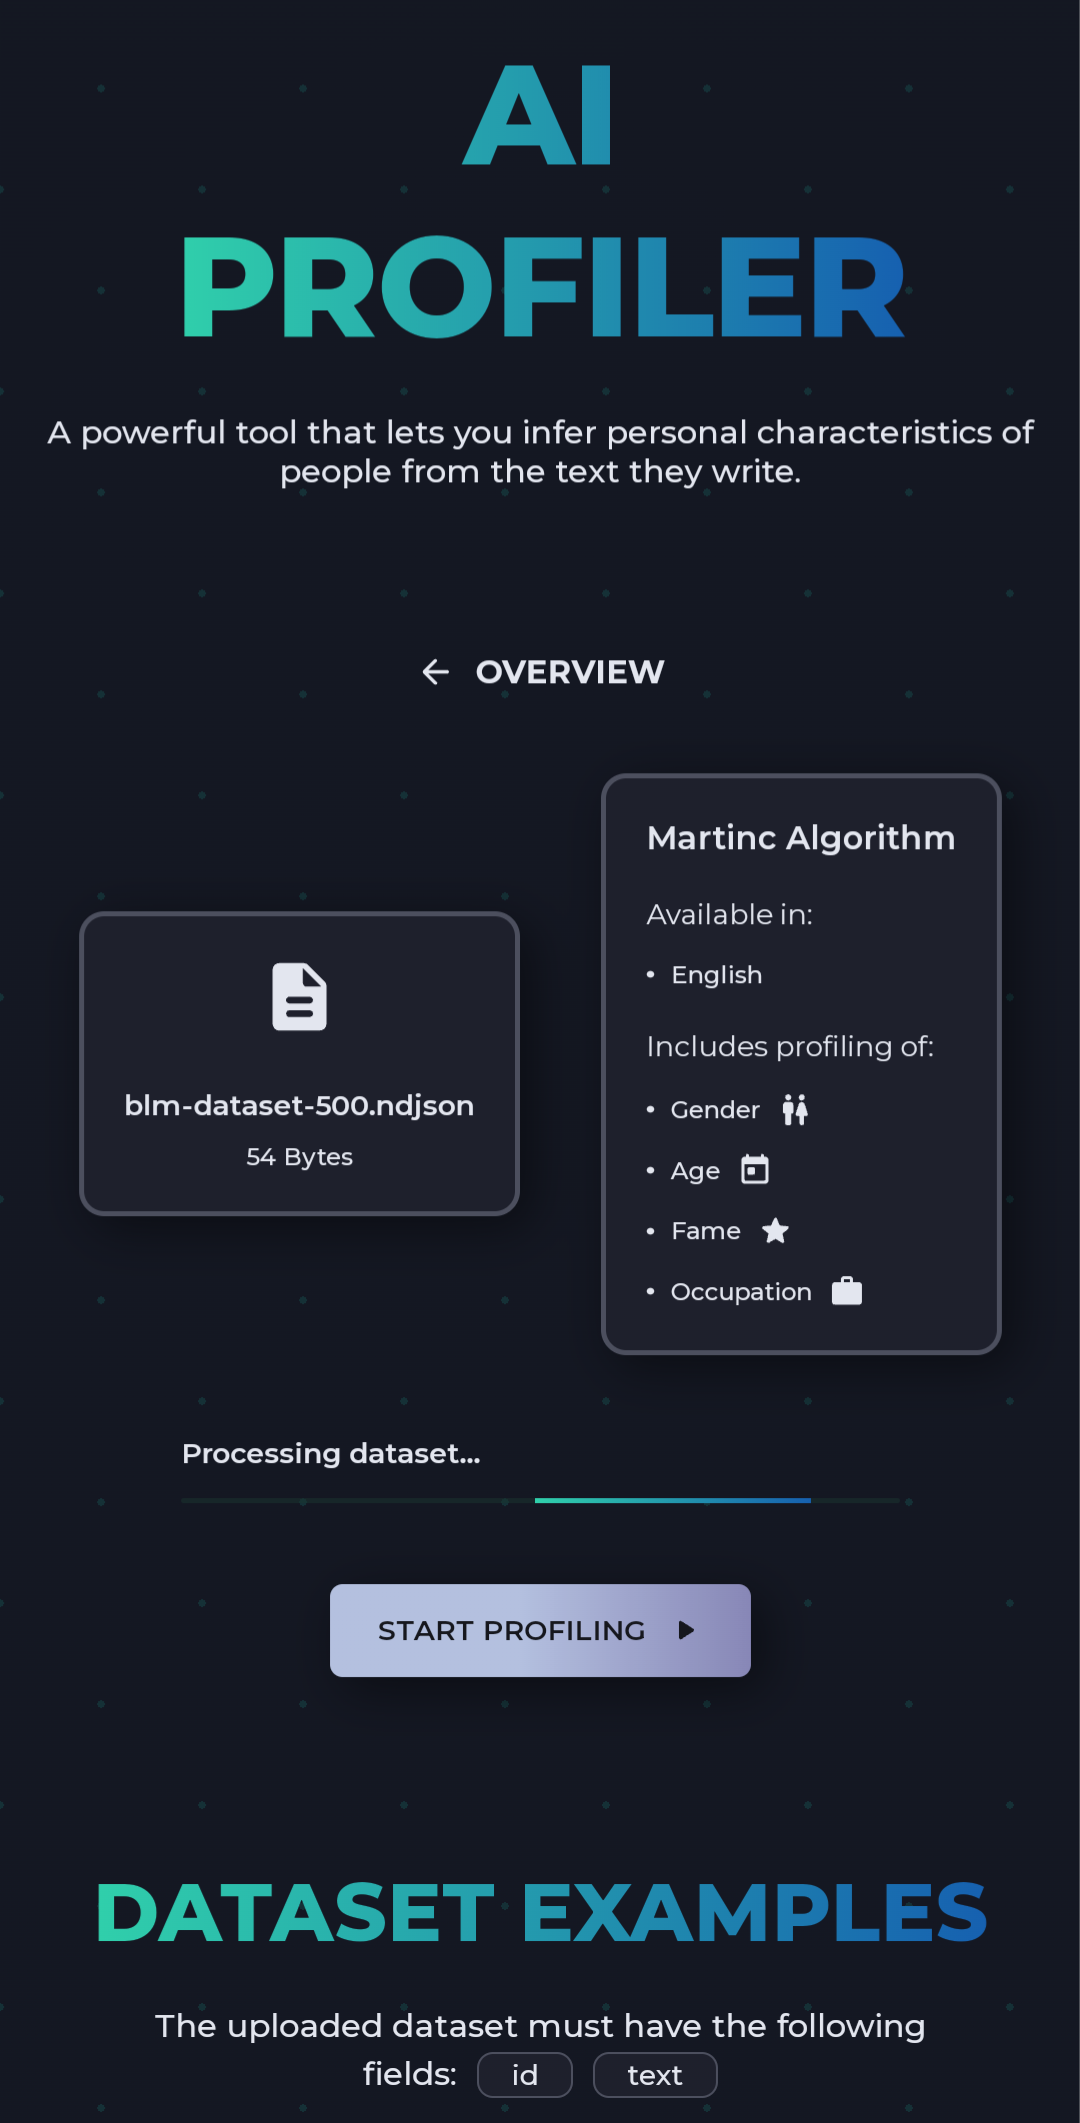
\includegraphics[width=\textwidth]{imagenes/overview_movil.png}
	% 		\label{fig:casouso_overview_movil}
	% \end{subfigure}
	\vspace{-1\baselineskip}
	\caption{Dashboard con los resultados obtenidos por el algoritmo de Grivas}
	\label{fig:casouso_dashboard_grivas}
\end{figure}

\section{Análisis de resultados}
